%iffalse
\let\negmedspace\undefined
\let\negthickspace\undefined
\documentclass[journal,12pt,onecolumn]{IEEEtran}
\usepackage{cite}
\usepackage{amsmath,amssymb,amsfonts,amsthm}
\usepackage{algorithmic}
\usepackage{graphicx}
\usepackage{textcomp}
\usepackage{xcolor}
\usepackage{txfonts}
\usepackage{listings}
\usepackage{enumitem}
\usepackage{enumitem,multicol}
\usepackage{mathtools}
\usepackage{gensymb}
\usepackage{comment}
\usepackage[breaklinks=true]{hyperref}
\usepackage{tkz-euclide} 
\usepackage{listings}
\usepackage{gvv}                                        
%\def\inputGnumericTable{}                                 
\usepackage[latin1]{inputenc}                                
\usepackage{color}                                            
\usepackage{array}                                            
\usepackage{longtable}                                       
\usepackage{calc}                                             
\usepackage{multirow}                                         
\usepackage{hhline}                                           
\usepackage{ifthen}                                           
\usepackage{lscape}
\usepackage{tabularx}
\usepackage{array}
\usepackage{float}
\usepackage[american,siunitx]{circuitikz}
\usetikzlibrary{arrows,shapes,calc,positioning}
\usepackage{pgfplots}


\newtheorem{theorem}{Theorem}[section]
\newtheorem{problem}{Problem}
\newtheorem{proposition}{Proposition}[section]
\newtheorem{lemma}{Lemma}[section]
\newtheorem{corollary}[theorem]{Corollary}
\newtheorem{example}{Example}[section]
\newtheorem{definition}[problem]{Definition}
\newcommand{\BEQA}{\begin{eqnarray}}
\newcommand{\EEQA}{\end{eqnarray}}
\newcommand{\define}{\stackrel{\triangle}{=}}
\theoremstyle{remark}
\newtheorem{rem}{Remark}
\pgfplotsset{compat=1.18}

% Marks the beginning of the document
\begin{document}
\bibliographystyle{IEEEtran}
\vspace{3cm}

\title{ME-2024}
\author{EE24Btech11022 - Eshan Sharma}
\maketitle

\renewcommand{\thefigure}{\theenumi}
\renewcommand{\thetable}{\theenumi}



\begin{enumerate}
\item Consider the system of linear equations
\begin{align*}
	x + 2y + z &= 5 \\
	2x + ay + 4z &= 12 \\
	2x + 4y + 6z &= b
\end{align*}
The values of $a$ and $b$ such that there exists a non-trivial null space and the system admits infinite solutions are
\begin{enumerate}
	\item $a = 8, \, b = 14$
	\item $a = 4, \, b = 12$
	\item $a = 8, \, b = 12$
	\item $a = 4, \, b = 14$
\end{enumerate}

\item Let $f(\cdot)$ be a twice differentiable function from $\mathbb{R}^2 \rightarrow \mathbb{R}$. If $p, x_0 \in \mathbb{R}^2$ where $\|p\|$ is sufficiently small (here $\|\cdot\|$ is the Euclidean norm or distance function), then 
\[
f(x_0 + p) = f(x_0) + \nabla f(x_0)^T p + \frac{1}{2} p^T \nabla^2 f(\psi) p
\]
where $\psi \in \mathbb{R}^2$ is a point on the line segment joining $x_0$ and $x_0 + p$. If $x_0$ is a strict local minimum of $f(x)$, then which one of the following statements is TRUE?
\begin{enumerate}
	\item $\nabla f(x_0)^T p > 0$ and $p^T \nabla^2 f(\psi) p = 0$
	\item $\nabla f(x_0)^T p = 0$ and $p^T \nabla^2 f(\psi) p > 0$
	\item $\nabla f(x_0)^T p = 0$ and $p^T \nabla^2 f(\psi) p < 0$
	\item $\nabla f(x_0)^T p = 0$ and $p^T \nabla^2 f(\psi) p = 0$
\end{enumerate}

\item The velocity field of a two-dimensional, incompressible flow is given by
\[
\vec{V} = 2 \sin h x \, \hat{i} + v(x, y) \, \hat{j}
\]
where $\hat{i}$ and $\hat{j}$ denote the unit vectors in $x$ and $y$ directions, respectively. If $v(x, 0) = \cos h x$, then $v(0, -1)$ is
\begin{enumerate}
	\item 1
	\item 2
	\item 3
	\item 4
\end{enumerate}

\item A plane, solid slab of thickness $L$, shown in the figure, has thermal conductivity $k$ that varies with the spatial coordinate $x$ as $k = A + B x$, where $A$ and $B$ are positive constants ($A > 0$, $B > 0$). The slab walls are maintained at fixed temperatures of $T(x = 0) = 0$ and $T(x = L) = T_0 > 0$. The slab has no internal heat sources. Considering one-dimensional heat transfer, which one of the following plots qualitatively depicts the steady-state temperature distribution within the slab?
\begin{center}
	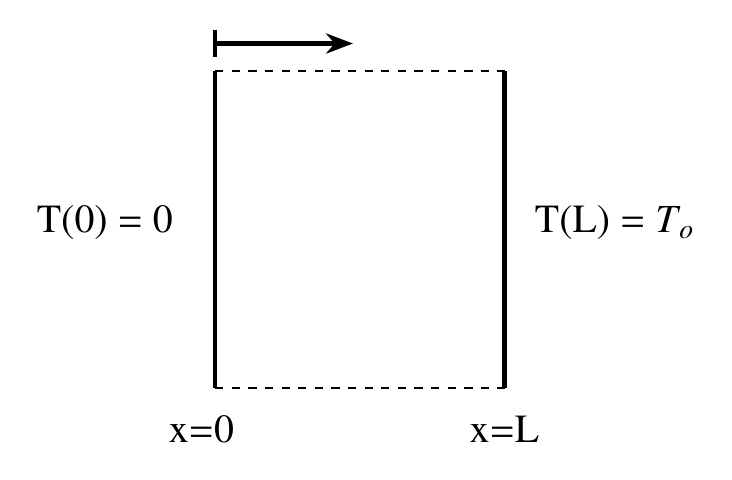
\begin{tikzpicture}[scale=0.7]
		\tikzstyle{every node}=[font=\Large]
		\draw [line width=1.5pt, short] (7.75,16.5) -- (7.75,10.75);
		\draw [line width=1.5pt, short] (13,16.5) -- (13,10.75);
		\draw [line width=1.5pt, short] (7.75,17.25) -- (7.75,16.75);
		\draw [line width=1.5pt, ->, >=Stealth] (7.75,17) -- (10.25,17);
		\draw [line width=1pt, dashed] (7.75,16.5) -- (13,16.5);
		\draw [line width=1pt, dashed] (7.75,10.75) -- (13,10.75);
		\node [font=\Large] at (5.75,13.75) {T(0) = 0};
		\node [font=\Large] at (15,13.75) {T(L) = $T_o$};
		\node [font=\Large] at (7.5,10) {x=0};
		\node [font=\Large] at (13,10) {x=L};
	\end{tikzpicture}
\end{center}

\begin{enumerate}
	\item 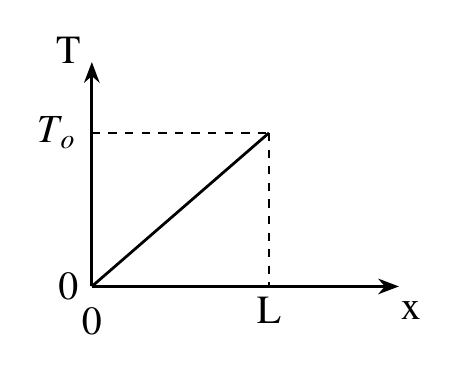
\begin{tikzpicture}[scale=0.6]
		\tikzstyle{every node}=[font=\Large]
		\draw [line width=1pt, ->, >=Stealth] (6.25,11.75) -- (6.25,16.5);
		\draw [line width=1pt, ->, >=Stealth] (6.25,11.75) -- (12.75,11.75);
		\draw [line width=1pt, short] (6.25,11.75) -- (10,15);
		\draw [line width=1pt, dashed] (6.25,15) -- (10,15);
		\draw [line width=1pt, dashed] (10,15) -- (10,11.75);
		\node [font=\Large] at (5.75,11.75) {0};
		\node [font=\Large] at (6.25,11) {0};
		\node [font=\Large] at (10,11.25) {L};
		\node [font=\Large] at (5.5,15) {$T_o$};
		\node [font=\Large] at (5.75,16.75) {T};
		\node [font=\Large] at (13,11.25) {x};
	\end{tikzpicture}
	\item 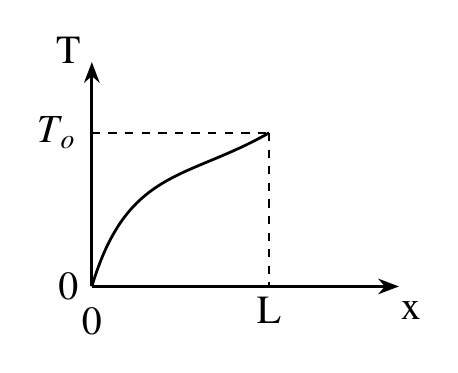
\begin{tikzpicture}[scale=0.6]
		\tikzstyle{every node}=[font=\Large]
		\draw [line width=1pt, ->, >=Stealth] (6.25,11.75) -- (6.25,16.5);
		\draw [line width=1pt, ->, >=Stealth] (6.25,11.75) -- (12.75,11.75);
		\draw [line width=1pt, short] (6.25,11.75) .. controls (7,14.25) and (8.25,14) .. (10,15);
		\draw [line width=1pt, dashed] (6.25,15) -- (10,15);
		\draw [line width=1pt, dashed] (10,15) -- (10,11.75);
		\node [font=\Large] at (5.75,11.75) {0};
		\node [font=\Large] at (6.25,11) {0};
		\node [font=\Large] at (10,11.25) {L};
		\node [font=\Large] at (5.5,15) {$T_o$};
		\node [font=\Large] at (5.75,16.75) {T};
		\node [font=\Large] at (13,11.25) {x};
	\end{tikzpicture}
	\item 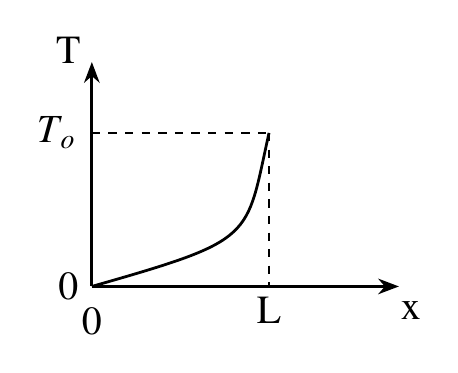
\begin{tikzpicture}[scale=0.6]
		\tikzstyle{every node}=[font=\Large]
		\draw [line width=1pt, ->, >=Stealth] (6.25,11.75) -- (6.25,16.5);
		\draw [line width=1pt, ->, >=Stealth] (6.25,11.75) -- (12.75,11.75);
		\draw [line width=1pt, short] (6.25,11.75) .. controls (9.75,12.75) and (9.5,12.75) .. (10,15);
		\draw [line width=1pt, dashed] (6.25,15) -- (10,15);
		\draw [line width=1pt, dashed] (10,15) -- (10,11.75);
		\node [font=\Large] at (5.75,11.75) {0};
		\node [font=\Large] at (6.25,11) {0};
		\node [font=\Large] at (10,11.25) {L};
		\node [font=\Large] at (5.5,15) {$T_o$};
		\node [font=\Large] at (5.75,16.75) {T};
		\node [font=\Large] at (13,11.25) {x};
	\end{tikzpicture}
	\item 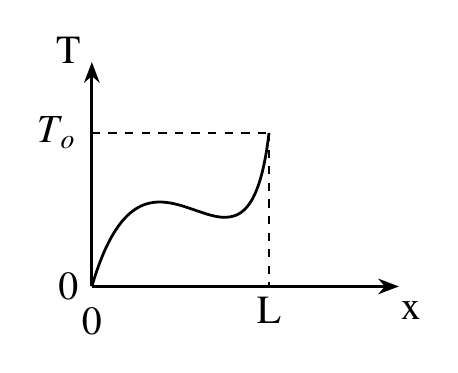
\begin{tikzpicture}[scale=0.6]
		\tikzstyle{every node}=[font=\Large]
		\draw [line width=1pt, ->, >=Stealth] (6.25,11.75) -- (6.25,16.5);
		\draw [line width=1pt, ->, >=Stealth] (6.25,11.75) -- (12.75,11.75);
		\draw [line width=1pt, short] (6.25,11.75) .. controls (7.5,16) and (9.5,10.75) .. (10,15);
		\draw [line width=1pt, dashed] (6.25,15) -- (10,15);
		\draw [line width=1pt, dashed] (10,15) -- (10,11.75);
		\node [font=\Large] at (5.75,11.75) {0};
		\node [font=\Large] at (6.25,11) {0};
		\node [font=\Large] at (10,11.25) {L};
		\node [font=\Large] at (5.5,15) {$T_o$};
		\node [font=\Large] at (5.75,16.75) {T};
		\node [font=\Large] at (13,11.25) {x};
	\end{tikzpicture}
\end{enumerate}

\item Consider incompressible laminar flow over a flat plate with freestream velocity of $u_{\infty}$. The Nusselt number corresponding to this flow velocity is $Nu_1$. If the freestream velocity is doubled, the Nusselt number changes to $Nu_2$. Choose the correct option for $Nu_2/Nu_1$.
\begin{enumerate}
	\item $\sqrt{2}$
	\item $2$
	\item $1.26$
	\item $1$
\end{enumerate}

\item Consider a hydrodynamically fully developed laminar flow through a circular pipe with the flow along the axis (i.e., $z$ direction). In the following statements, $T$ is the temperature of the fluid, $T_w$ is the wall temperature, and $T_m$ is the bulk mean temperature of the fluid. Which one of the following statements is TRUE?
\begin{enumerate}
	\item For a thermally fully developed flow, $\frac{\partial T}{\partial z} = 0$, always.
	\item For constant wall temperature of the duct, $\frac{d T_m}{d z} =$ constant.
	\item Nusselt number varies linearly along the $z$ direction for a thermally fully developed flow.
	\item For constant wall temperature $(T_w > T_m)$ of the duct, $\frac{d T_m}{d z}$ increases exponentially with distance along $z$ direction.
\end{enumerate}

\item A furnace can supply heat steadily at 1200 K at a rate of 24000 kJ/min. The maximum amount of power (in kW) that can be produced by using the heat supplied by this furnace in an environment at 300 K is
\begin{enumerate}
	\item 300
	\item 150
	\item 18000
	\item 0
\end{enumerate}

\item Which one of the following statements regarding a Rankine cycle is FALSE?
\begin{enumerate}
	\item Superheating the steam in the boiler increases the cycle efficiency.
	\item The pressure at the turbine outlet depends on the condenser temperature.
	\item Cycle efficiency increases as condenser pressure decreases.
	\item Cycle efficiency increases as boiler pressure decreases.
\end{enumerate}

\item For a ball bearing, the fatigue life in millions of revolutions is given by 
\[
L = \left(\frac{C}{P}\right)^n,
\]
where $P$ is the constant applied load and $C$ is the basic dynamic load rating. Which one of the following statements is TRUE?
\begin{enumerate}
	\item $n = 3$, assuming that the inner race is fixed and the outer race is revolving
	\item $n = \frac{1}{3}$, assuming that the inner race is fixed and the outer race is revolving
	\item $n = 3$, assuming that the outer race is fixed and the inner race is revolving
	\item $n = \frac{1}{3}$, assuming that the outer race is fixed and the inner race is revolving
\end{enumerate}

\item The change in kinetic energy $\Delta E$ of an engine is 300 J, and minimum and maximum shaft speeds are $\omega_{\min} = 220 \, \text{rad/s}$ and $\omega_{\max} = 280 \, \text{rad/s}$, respectively. Assume that the torque-time function is purely harmonic. To achieve a coefficient of fluctuation of 0.05, the moment of inertia (in kg.m$^2$) of the flywheel to be mounted on the engine shaft is
\begin{enumerate}
	\item 0.113
	\item 0.096
	\item 0.071
	\item 0.053
\end{enumerate}

\item A ram in the form of a rectangular body of size $l = 9$ m and $b = 2$ m is suspended by two parallel ropes of lengths 7 m. Assume the center-of-mass of the body is at its geometric center and $g = 9.81$ m/s$^2$. For striking the object $P$ with a horizontal velocity of 5 m/s, what is the angle $\theta$ with the vertical from which the ram should be released from rest?

\begin{center}
	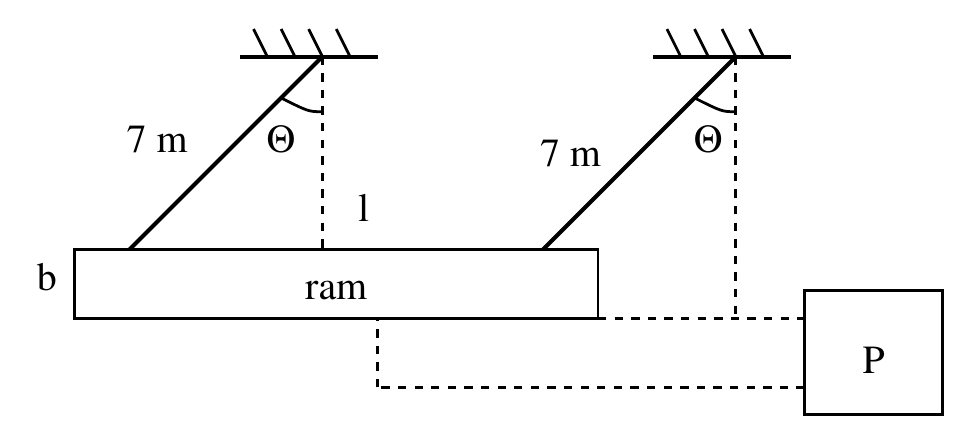
\begin{tikzpicture}[scale=0.7]
		\tikzstyle{every node}=[font=\Large]
		\draw [line width=1.5pt, short] (6,15.25) -- (8.5,15.25);
		\draw [line width=1.5pt, short] (13.5,15.25) -- (16,15.25);
		\draw [line width=1.5pt, short] (7.5,15.25) -- (4,11.75);
		\draw [line width=1.5pt, short] (15,15.25) -- (11.5,11.75);
		\draw [ line width=1pt ] (3,11.75) rectangle (12.5,10.5);
		\draw [line width=1pt, dashed] (7.5,15.25) -- (7.5,11.75);
		\draw [line width=1pt, dashed] (15,15.25) -- (15,10.5);
		\draw [line width=1pt, dashed] (12.5,10.5) -- (16.25,10.5);
		\draw [line width=1pt, dashed] (16.25,10.5) -- (16.25,9.25);
		\draw [line width=1pt, dashed] (16.25,9.25) -- (8.5,9.25);
		\draw [line width=1pt, dashed] (8.5,9.25) -- (8.5,10.5);
		\draw [ line width=1pt ] (16.25,11) rectangle (18.75,8.75);
		\node [font=\Large] at (7.75,11) {ram};
		\node [font=\Large] at (17.5,9.75) {P};
		\node [font=\Large] at (4.5,13.75) {7 m};
		\node [font=\Large] at (12,13.5) {7 m};
		\draw [line width=1pt, short] (6.75,14.5) .. controls (7.25,14.25) and (7.25,14.25) .. (7.5,14.25);
		\draw [line width=1pt, short] (14.25,14.5) .. controls (14.75,14.25) and (14.75,14.25) .. (15,14.25);
		\node [font=\Large] at (6.75,13.75) {$\Theta$};
		\node [font=\Large] at (14.5,13.75) {$\Theta$};
		\draw [line width=1pt, short] (6.25,15.75) -- (6.5,15.25);
		\draw [line width=1pt, short] (6.75,15.75) -- (7,15.25);
		\draw [line width=1pt, short] (7.25,15.75) -- (7.5,15.25);
		\draw [line width=1pt, short] (7.75,15.75) -- (8,15.25);
		\draw [line width=1pt, short] (13.75,15.75) -- (14,15.25);
		\draw [line width=1pt, short] (14.25,15.75) -- (14.5,15.25);
		\draw [line width=1pt, short] (14.75,15.75) -- (15,15.25);
		\draw [line width=1pt, short] (15.25,15.75) -- (15.5,15.25);
		\node [font=\Large] at (8.25,12.5) {l};
		\node [font=\Large] at (2.5,11.25) {b};
	\end{tikzpicture}
\end{center}

\begin{enumerate}
	\item $67.1^\circ$
	\item $40.2^\circ$
	\item $35.1^\circ$
	\item $79.5^\circ$
\end{enumerate}

\item A linear spring-mass-dashpot system with a mass of 2 kg is set in motion with viscous damping. If the natural frequency is 15 Hz, and the amplitudes of two successive cycles measured are 7.75 mm and 7.20 mm, the coefficient of viscous damping (in N.s/m) is
\begin{enumerate}
	\item 4.41
	\item 7.51
	\item 2.52
	\item 6.11
\end{enumerate}

\item Which one of the following failure theories is the most conservative design approach against fatigue failure?
\begin{enumerate}
	\item Soderberg line
	\item Modified Goodman line
	\item Gerber line
	\item Yield line
\end{enumerate}
\end{enumerate}
\end{document}


